\documentclass{kththesis}

\usepackage[export]{adjustbox}
\usepackage{amsmath}
\usepackage[style=numeric,sorting=none,backend=biber]{biblatex}
\usepackage{booktabs}
\usepackage{caption}
\usepackage{csquotes} % Recommended by biblatex
\usepackage[super]{nth}
\usepackage{relsize}
\usepackage{siunitx}
\usepackage{subcaption}
\usepackage{wrapfig}

\addbibresource{references.bib} % The file containing our references, in BibTeX format
\renewcommand{\arraystretch}{1.2}
\newcommand{\source}[1]{\vspace{-5mm}\caption*{\textcolor{darkgray}{Author: {#1}}\vspace{-7mm}} }
\captionsetup[table]{skip=10pt}

\title{Evaluating a simple convolutional neural network for classifying Alzheimer's disease}
\alttitle{Utvärdering av ett enkelt CNN-nätverk för klassifiering av Alzheimers sjukdom}
\author{Karl Lundstig}
\email{lundsti@kth.se}
\supervisor{Jeanette Hällgren Kotaleski}
\examiner{Örjan Ekeberg}
\programme{Degree Project in Computer Science, DD142X}
\school{School of Electrical Engineering and Computer Science}
\date{\today}

% Uncomment the next line to include cover generated at https://intra.kth.se/kth-cover?l=en
\kthcover{kth-cover.pdf}


\begin{document}

% Frontmatter includes the titlepage, abstracts and table-of-contents
\frontmatter

\titlepage

\begin{abstract}
  English abstract goes here.
  $$\int \gamma$$

\end{abstract}


\begin{otherlanguage}{swedish}
  \begin{abstract}
    Träutensilierna i ett tryckeri äro ingalunda en oviktig faktor,
    för trevnadens, ordningens och ekonomiens upprätthållande, och
    dock är det icke sällan som sorgliga erfarenheter göras på grund
    af det oförstånd med hvilket kaster, formbräden och regaler
    tillverkas och försäljas Kaster som äro dåligt hopkomna och af
    otillräckligt.
  \end{abstract}
\end{otherlanguage}


\setcounter{secnumdepth}{2}
\setcounter{tocdepth}{2}
\tableofcontents


% Mainmatter is where the actual contents of the thesis goes
\mainmatter

\chapter{Introduction}

In the last couple of years machine learning and specifically deep learning have been applied successfully on several problems such as speech recognition, image recognition \parencite{krizhevsky2012imagenet}, and even board games \parencite{silver2018general}. One area which could benefit greatly from effective image recognition and analysis is medical diagnostics.

Alzheimer’s Disease (AD) is a neurodegenerative disease that is the leading cause of dementia. There is currently no cure, but early detection is still important as it can be beneficial to the patient~\cite{factsfigures2018}.

Many studies~\cite{islam2017novel, islam2018early} shows promising results for identifying and classifying Alzheimer’s Disease using structural MRI data, using mainly the OASIS\cite{oasis} or ADNI\cite{adni} datasets.

\section{Research Question}
This study will not try to acheive state-of-the-art results on Alzheimer's disease diagnosis; instead the goal is to evaluate the performance of a simple CNN model on medical data when using various training schemes. The model's accuracy will be measured starting from the simplest strategy, and then various improvements will be incrementally added and evaluated.

\section{Acknowledgments}
Data were provided by OASIS-3: Principal Investigators: T. Benzinger, D. Marcus, J. Morris; NIH P50AG00561, P30NS09857781, P01AG026276, P01AG003991, R01AG043434, UL1TR000448, R01EB009352. AV-45 doses were provided by Avid Radiopharmaceuticals, a wholly owned subsidiary of Eli Lilly.

\chapter{Background}

\section{Alzheimer's Disease}

Dementia is a group of symptoms that may have many different causes. Alzheimer's disease is a degenerative brain disease, estimated to be the cause of 60\% to 80\% of dementia cases. In half of these cases Alzheimer's is the only cause, while many other also have evidence of other dementia causing changes~\cite{factsfigures2018}.

Early (and accurate) diagnosis of Alzheimer's disease has several benefits. Those who do not have Alzheimer's but are diagnosed with mild cognitive impairment, might after testing realize that they're suffering from some other, treatable condition. There are also medical and social benefits to get an Alzheimer's diagnosis early. Neither a curing nor a slowing treatment exist, but individuals can still take measures to retain ther cognitive function for as long as possible. Aerobic exercise, mental activity and social engagement may help delay cognitive decline, while medication and other intervention can help with managing symptoms. An early diagnosis can also help reduce anxiety by giving noticed symptoms a name, for both affected individuals and their family members. Finally, early diagnosis gives individuals time to make plans for the future while still having good cognitive function~\cite[p. 406-409]{factsfigures2018}.

\subsection{Symptoms}
Individuals with Alzheimer's disease can experience multiple and varying symptoms, which change over several years~\cite{factsfigures2018}.

\subsection{Benefits of early detection}
Early (and accurate) diagnosis of Alzheimer's disease has several benefits. Those who do not have Alzheimer's but are diagnosed with mild cognitive impairment, might after testing realize that they're suffering from some other, treatable condition. There are also medical and social benefits to get an Alzheimer's diagnosis early. Neither a curing nor a slowing treatment exist, but individuals can still take some measures that helps them retain their cognitive function for as long as possible. Aerobic exercise, mental activity and social engagement may help delay cognitive decline, while medication and other intervention can help with managing symptoms. An early diagnosis can also help reduce anxiety by giving noticed symptoms a name, for both affected individuals and their family members. Finally, early diagnosis gives individuals time to make plans for the future while still having good cognitive function~\cite[p. 406-409]{factsfigures2018}.

\subsection{Brain changes}
The abnormal accumulation of two proteins (what is called beta-amyloid plaques and tau tangles) inside the brain is one of several brain changes associated with Alzheimer's disease. These proteins interfer with neuron communication and nutrient transportation, while also triggering inflammation. Brain shrinkage, or \textit{atrophy,} eventually occurs because of cell loss. These changes may start as early as 20 years or more before symptoms appear~\cite{factsfigures2018}.

Brain atrophy occurs in a relatively late disease stage, when neurodegeneration has started to occur. This atrophy can be detected and measured using MRI imaging, and is a medically established predictor of an individual progressing from mild cognitive impairement to Alzheimer's disease. In addition there seems to be a direct relationship between the severity of the atrophy and time-to-dementia. Brain atrophy is, however, not a unique sign of Alzheimer's but a measure of neural degeneration in general, degeneration which might be caused by other conditions~\cite{jack2010brain}.

\subsection{Clinical dementia rating}
Clinical dementia rating (CDR) is a mesure of

\section{Machine learning}
\subsection{Artificial neural networks}
\subsubsection{Introduction}
Artificial neural networks (ANNs) are computational modeling tools inspired by the neural networks found in biology. ANNs exhibit several information processing characteristics which make them useful for modeling complex real-word problems, among them non-linearity, their ability to handle imprecise information, and their ability to generalize~\cite{ANNFundamentals}. A common machine learning task is \textit{classification}. Here the machine learning algorithm is presented with a dataset containing many datapoints, each having some number of features and an assigned class. The goal of the machine learning model is then to learn a mapping from features to class, such that the model can be applied to new data where the class is unknown. ANNs are often used successfully for this task, but they do have the drawback that the models are opaque, or in other words they can't reason about why they give the output that they do~\cite[p. 3, 8--9]{weiss1990empirical}.

\begin{figure}
  \begin{center}
    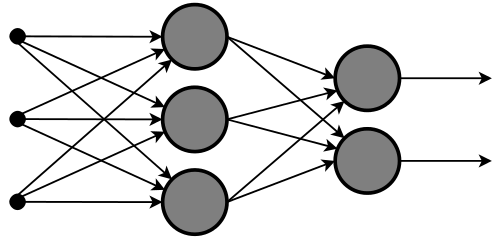
\includegraphics[width=100mm]{img/neural_network.png}
    \caption{An illustration of a multi-layer artifical neural network. }
    \source{Offnfopt / CC-BY-SA 3.0.}
    \label{fig:mlf}
  \end{center}
\end{figure}

\subsubsection{Structure}
Artificial neural networks can be constructed in different ways, but the most common is the so called \textit{multi-layer feed-forward neural network}, illustrated in Figure~\ref{fig:mlf}. It consists of neurons ordered into multiple layers, the first layer being the \textit{input layer} and the last one the \textit{output layer}. The layers in between are called \textit{hidden layers}. Each neuron is connected with all the neurons in the next layer, with every connection from neuron $i$ to neuron $j$ having a weight coefficient $w_{ij}$. In addition, every neuron has a threshhold coefficient, or bias $b_i$. Using these coefficients and all the inputs from the previous layer, every neuron produces an output $x_i$, which can be formally written as follows:
\[x_i = \mathlarger{\varphi}\left(\sum_{j \in \Gamma^{-1}(i)}{w_{ij} \cdot x_j}\right)\]

Here $\Gamma^{-1}(i)$ is notation for the set of all neurons in the previous layer, and $\varphi$ is some \textit{activation function} which squeezes the weighted sum of all input neurons into the range $[0, 1]$, in preparation of passing the output along to the next neuron~\cite{mlfIntro}.j

\subsubsection{Activation functions}
There are many possible choices for the activation function, but three of the most common ones can be found in Table~\ref{tab:activation_functions}. The softmax activation function is a little different than the others since it doesn't work on only one neuron, but instead on all neurons in the layer. In doing this, the softmax function can ensure that the sum of all the output values are equal to $1$, which is a desirable thing for the output layer when classifying into $K$ different classes. This also allows the use the \textit{cross-entropy error function} (see later section), which seems to give higher accuracy than using the sigmoid function and the \textit{least squares error function}~\cite{dunne1997pairing}.

\begin{table}[h]
  \renewcommand{\arraystretch}{1.2}
  \begin{center}
    \caption{Selection of common activation functions.}
    \label{tab:activation_functions}
    \begin{tabular}{cc}
      \textbf{Name} & \textbf{Function} $\varphi(x)$\\
      \toprule
      Sigmoid & $\displaystyle \frac{1}{1 + e^{-x}} $ \\[4mm]
      Rectifier & $\displaystyle \max(0, x)$ \\[3mm]
      Softmax & $\displaystyle \frac{e^{x_i}}{\sum_j^K{e^{x_j}}}$ \\
    \end{tabular}
  \end{center}
\end{table}

\subsubsection{Error functions}
To be able to train our network, we need some way to determine how `bad' a certain output is. This is done using an \textit{error function}, or \textit{loss function}. This function is averaged on the network's output on all training samples. In a classification task, the averaged loss being low means that the network is good at predicting the correct class given a certain input data. If the network performs perfectly, the error function is generally $0$. \textit{Least squares error} is a traditional error function, and if you let $x$ and $\hat{x}$ be the network's output and the wanted output respectively, the least squares error is defined as~\cite{mlfIntro}:

\[ E = \sum_i{\frac{1}{2}(x_i - \hat{x}_i)^2} \] 

There is however also another error function that was mentioned earlier, the \textit{cross-entropy error} function. This has some theoretical advantages over least squares error, such as better handling when the probabilities estimated by the network is small, as well as being less dominated by large outliers. Experiments also suggest that these advantages are large enough to be useful in practice~\cite{crossentropy_squared}. The cross-entropy is defined like this:

\[ E = \sum_i{\hat{x}_i\left(\frac{x_i}{\hat{x}_i}\right)} \]

\subsubsection{Gradient descent}
\begin{wrapfigure}{r}{0.3\linewidth}
  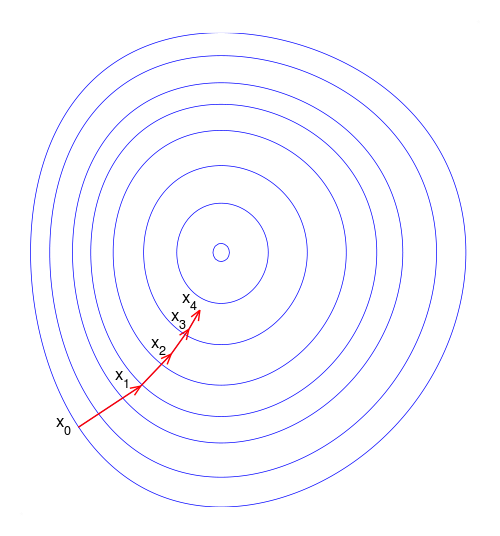
\includegraphics[width=1.6\linewidth]{img/gradient_descent.png}
\end{wrapfigure}
To train a neural network, we want to change the weights and biases (the network's parameters) such that the error on the training set becomes as low as possible. This is done using a process called \textit{gradient descent}. Given the error function and the dataset, the neural network can be viewed a giant function, taking all the parameters as input. By finding the slope or \textit{gradient} of the parameters in the direction that decreases the error, the parameters can gradually be adjusted to find a minimum of the error function. Since this gradient is calculated using the entire dataset to perform a single step, it is known as \textit{batch} gradient descent. Due to this batch gradient descent can become very slow on large datasets, and does not work at all if the dataset does not fit in memory~\cite{gradient_descent}

Because of this a variant of gradient descent named \textit{stochastic} gradient descent (SGD) is sometimes used, where the gradient is calculated using only a single training example at a time. This makes updates to the parameters much faster, but also causes the error function to jump around. This fluctuation adds noise, but also helps the model to not get stuck in local minima. SGD also has the benefit of allowing online learning, where the network can train on new data as it becomes available. In addition the overhead of calculating the gradient this many times might have a negative influence on the final perfomance~\cite{gradient_descent}.

There is also a third option, \textit{mini-batch} gradient descent, which aims to combine the best of both batch and stochastic gradient descent. Here the gradient calculation is performed on \textit{mini-batches} of $n$ training examples. This can help by making the updates more stable, and also helps with utilizing optimized matrix libraries that enables quickly calculating the gradient for a mini-batch. This is the method typically used when training neural networks in practice, and the term SGD is usually used to refer to this method as well~\cite{gradient_descent}.

\subsubsection{Learning rate}
The learning rate is a parameter that determines how large steps should be taken when performing the gradient descent. Too large a learning rate, and the network will not converge. Too small, and the convergence will take too long. A common strategy is to keep decreasing the learning rate as training progresses~\cite{Bottou2012}.

\subsection{Convolutional neural networks}

\subsubsection{Motivation}
One of the largest limitations of traditional artificial neural networks is that they struggle with the complexity of images. The input of a grayscale image of just $112 \times 112$ pixels require \num{12544} connections for every neuron in the first hidden layer! This means that the network has to have a very large number of parameters, which results in training of the network becoming very computationally demanding, as well as increasing the chances of overfitting. A model with fewer parameters to train makes overfitting less likely, which improves the network's performance~\cite{cnnIntro}.

\subsubsection{Structure}
Convolutional neural networks (CNNs) are specifically designed to work with images as input, and therefore has a different structure than traditional neural networks.
The neurons in a layer are not connected to the all neurons in the preceding layer, instead only connecting to a small region of it.
CNNs have three different types of layers: \textit{convolutional} layers, \textit{pooling} layers, and \textit{fully-connected} layers.
The layers are said to have three dimensions: height, width, and depth. The initial height and width correspond to the input image dimensions, while the depth represents different \textit{feature maps}.
If the images the network trains on are grayscale and has size $112 \times 112$, the input `volume' will have the dimension $(112, 112, 3)$~\cite{cnnIntro}.

\subsubsection{Convolutional layers}
Convolutional layers consists of a number of different \textit{filters}. These filters usually have small dimensions, say $(3, 3)$, but works on the entire depth of the input and are used to sweep, or \textit{convolve}, over the input's width and height. A $3 \times 3$ filter would have $3 \times 3 \times depth$ adjustable parameters, which forms the filter's \textit{kernel}. The output value, which will be located at the pixel in the center of the filter, is the dot product of the kernel and the current input region~\cite{cnnIntro}. For an illustration of this see Figure~\ref{fig:cnn_color_filter}.

\begin{figure}
  \begin{center}
    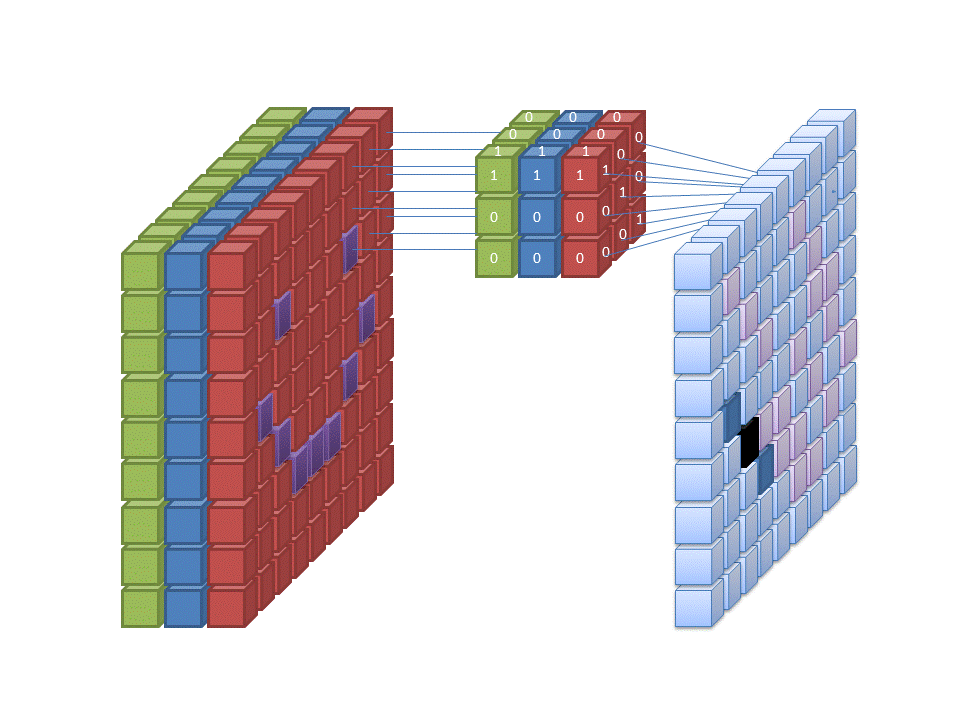
\includegraphics[width=100mm]{img/cnn_color_filter.png}
    \caption{Illustration of a filter on a color image.}
    \source{Cecbur / CC-BY-SA 4.0.}
    \label{fig:cnn_color_filter}
  \end{center}
\end{figure}

The depth of a layer's output volume in the CNN can be increased by increasing the number of filters used. The filters can pick up on different features, of which the intensity in different regions of the image will be outputted in the different depth dimensions, and picked up by later layers.

Another parameter that can be adjusted for the layer is the \textit{stride}. A stride of $1$ means that the filter is moved one step at a a time, while a higer stride of $n$ can be used to make the filter only evaluate every $n^{\text{th}}$ possible possition. This reduces overlap, but has the benefit of shrinking the output volume.

For filters of size larger than $1 \times 1$, the output will have slightly smaller dimensions since the filter can't go outside the edge of the input. To avoid missing features on the edges, \textit{zero-padding} is often used. This pads the input volume with enough zeroes to make the output volume the correct size, enabling the filter to be positioned right on the edge~\cite{cnnIntro}.

\subsubsection{Pooling layers}
A different way of shrinking the layers' spatial dimension are \textit{pooling layers}. These are used to gradually reduce the representation's dimensionality, which reduces the total amount of parameters that need to be trained. The most common method is by using $2\times 2$ max-pooling layer. This is applied with stride 2 on the input volume, shrinking the output width and height by 2 and reducing the total output size to 25~\%. As the name implies, the output value is simply the maximum of the input values in the region as shown in Figure~\ref{fig:max_pooling}. Pooling retains the number of depth dimensions~\cite{cnnIntro}.

\begin{figure}
  \begin{center}
    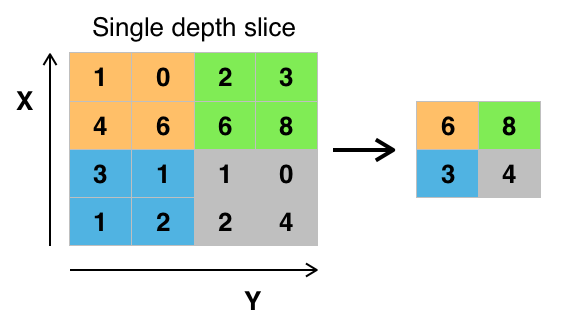
\includegraphics[width=80mm]{img/max_pooling.png}
    \caption{Example of max pooling.}
    \source{Aphex34 / CC-BY-SA 4.0.}
    \label{fig:max_pooling}
  \end{center}
\end{figure}

\subsubsection{Fully-connected layers}
The fully connected layers work just like they do in traditional neural networks, and are often placed at the end of a CNN network. This lets them compact all the data in the final volume into the final output of the network.

\subsubsection{Common architectures}
Commonly a CNN is constructed by stacking pairs of convolutional and pooling layers, before finally ending with fully-connected layers. This convolutional outputs are passed through the rectifier activation function. Another common option is to have two convolution layers before the pooling layers. This is recommended since it allows the network to learn more complicated features. The general trend in the layer volume dimensions is that they become smaller but deeper towards the end of the network~\cite{cnnIntro}. For an illustration of a complete CNN architecture, see Figure~\ref{fig:typical_cnn}.

\begin{figure}
  \begin{center}
    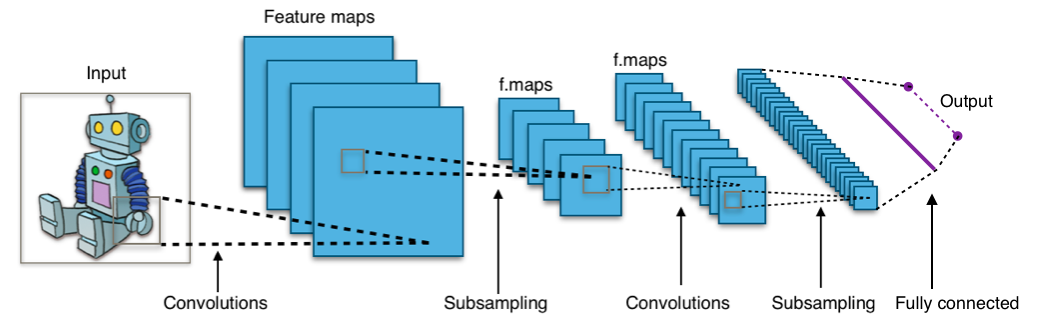
\includegraphics[width=150mm]{img/typical_cnn.png}
    \caption{Illustration of a typical CNN architecture.}
    \source{Aphex34 / CC-BY-SA 4.0.}
    \label{fig:typical_cnn}
  \end{center}
\end{figure}

\subsubsection{Gradient ascent in input space}

\section{Previous work}
Zhang and co.
This was done using a version of a convolutional neural network (CNN) trained on the OASIS dataset \parencite{oasis}. While their model showed acceptable performance for identifying non-demented patients, its performance on classifying demented patients was significantly worse, which could be because of the limited number of samples.

\chapter{Methods}

I will in this study recreate the convolutional neural network used in the second study by Islam and Zhang

OASIS-3 is a longitudinal neuroimaging dataset, with data collected over the course of 30 years from 1098 participants in various projects. Of these participants 809 were cognitively normal adults, while 489 were at various stages of cognitive decline. Accompanying the neural imaging is (among other things) clinical assessments of cognitive function~\cite{oasis3}. I will use the T1-weighted brain scans and mental assessments which were done using the CDR system. The dataset in total contains 3393 T1-weighted MRI images and 4089 different CDR evaluations.

\section{Labeling}
I will use the assessment of the subjects CDR score to label every MRI image with the stage of dementia. However, since OASIS-3 is a longitudinal study, the MRI scans and the clinical assessments were not performed at the same time. In fact, the time between MRI scans and the closest CDR assessment can be relatively large ($\mu=116$, $\sigma=107$). The distribution is shown in Figure~\ref{fig:mri_cdr_offset}. For most of the data the time from an MRI scan to the closest CDR assessment is less than 200 days, while for some images the delay can be several hundred days.

To try to get reasonable CDR labels even when the time offsets are high, a linear interpolation of the two closest CDR assessments and the time of the MRI scan will be used when this is possible. If the MRI scan was done either before or after all of this subjects' CDR assessments, the MRI scan will simply be tagged with the closest one.

The CDR calculation can be written as follows:
\begin{flalign*}
  \begin{aligned}
    \text{cdr} &=
    \begin{cases}
      \text{cdr}_{\text{next}}   & \text{if before all assessments} \\
      \text{cdr}_{\text{prev}} & \text{if after all assessments} \\
      \text{cdr}_{\text{prev}} + x * (\text{cdr}_{\text{next}} - \text{cdr}_{\text{prev}}) & \text{otherwise} \\
    \end{cases} & \\[5pt]
    \text{where }x &= \frac{\text{day}_{\text{MRI}} - \text{day}_\text{prev}}{\text{day}_{\text{prev}} - \text{day}_{\text{next}}}&
  \end{aligned}
\end{flalign*}

Here $0 \leq x \leq 1$ is the interpolation factor between the two assessments closest to $\text{day}_{\text{MRI}}$, the day the MRI scan was done.

\begin{figure}
  \begin{center}
    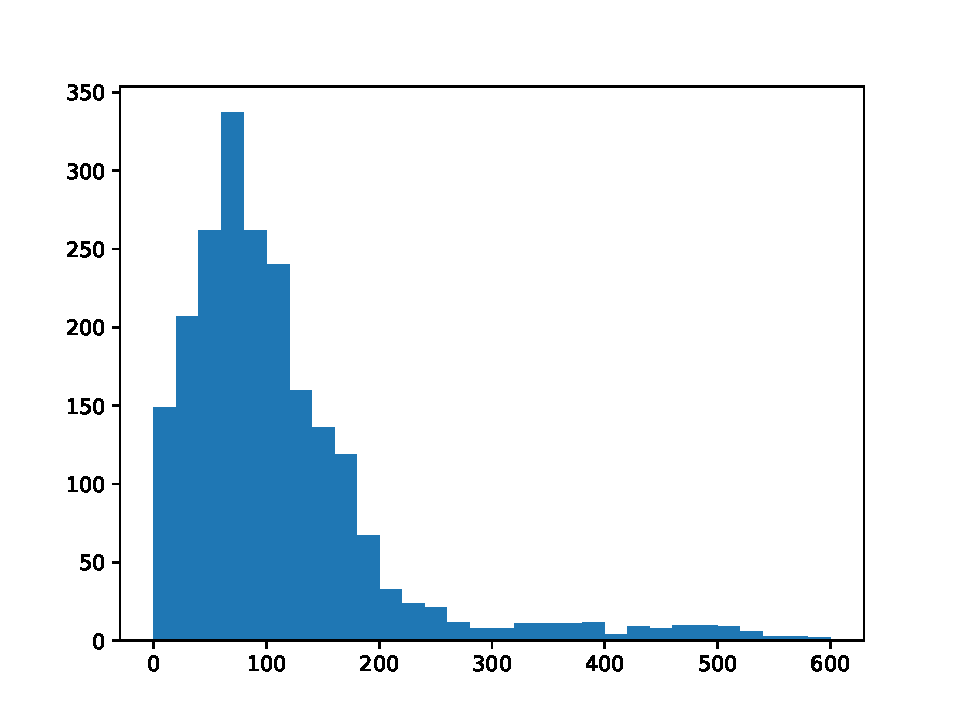
\includegraphics[width=100mm]{img/mri_cdr_offset.pdf}
    \caption{Histogram of time between MRI scans and the closest CDR assessment (in days).}
    \label{fig:mri_cdr_offset}
  \end{center}
\end{figure}

\section{Image extraction}
During the preprocessing step the three image planes are extracted from each MRI scan. For simplicity the planes chosen are simply the middle one for each axis, and the raw intensity values from each scan are flattened into the normal black/white range of PNG images.

Some scans are rotated the wrong way, even after realigning the images when loading. These images are simply skipped for now.

\section{Dataset contents}
The dataset in total contains 2782 images (ignoring the wrongly rotated ones). Of these images 20~\% were selected to be used as validation data, while the other 80~\% will be used to train the network. Just as in the paper by \textcite{islam2018early} I will use the CDR scores to divide the images into four classes: \textit{non-demented}, \textit{very mild dementia}, \textit{mild dementia}, and \textit{moderate dementia}. These classes are not equally represented in the dataset, with the more serious dementia cases being much less frequent. The total count of each case is shown in Table~\ref{tab:dataset_contents}, with the count in training and verification broken out.

\begin{table}[h]
  \begin{center}
    \caption{Count of images belonging to each class in the dataset.\label{tab:dataset_contents}}
    \begin{tabular}{r|cccc}
      \textbf{CDR Class} & \textbf{Total} & \textbf{Training set} & \textbf{Verification set} \\
      \toprule
      Non-demented (0.0) & 2163 & 1787 & 376 \\
      Very mild (0.5) & 443 & 357 & 86 \\
      Mild (1.0) & 153 & 120 & 33 \\
      Moderate (2.0) & 23 & 18 & 5 \\
    \end{tabular}
  \end{center}
\end{table}

\newpage
\section{Network structure}
\begingroup
\setlength{\columnsep}{0pt}%
\setlength\intextsep{0mm}
\begin{wrapfigure}{l}{0.3\linewidth}
  % \adjustimage{width=.3\textwidth,left}{img/model.pdf}
  \hspace*{-30mm}
  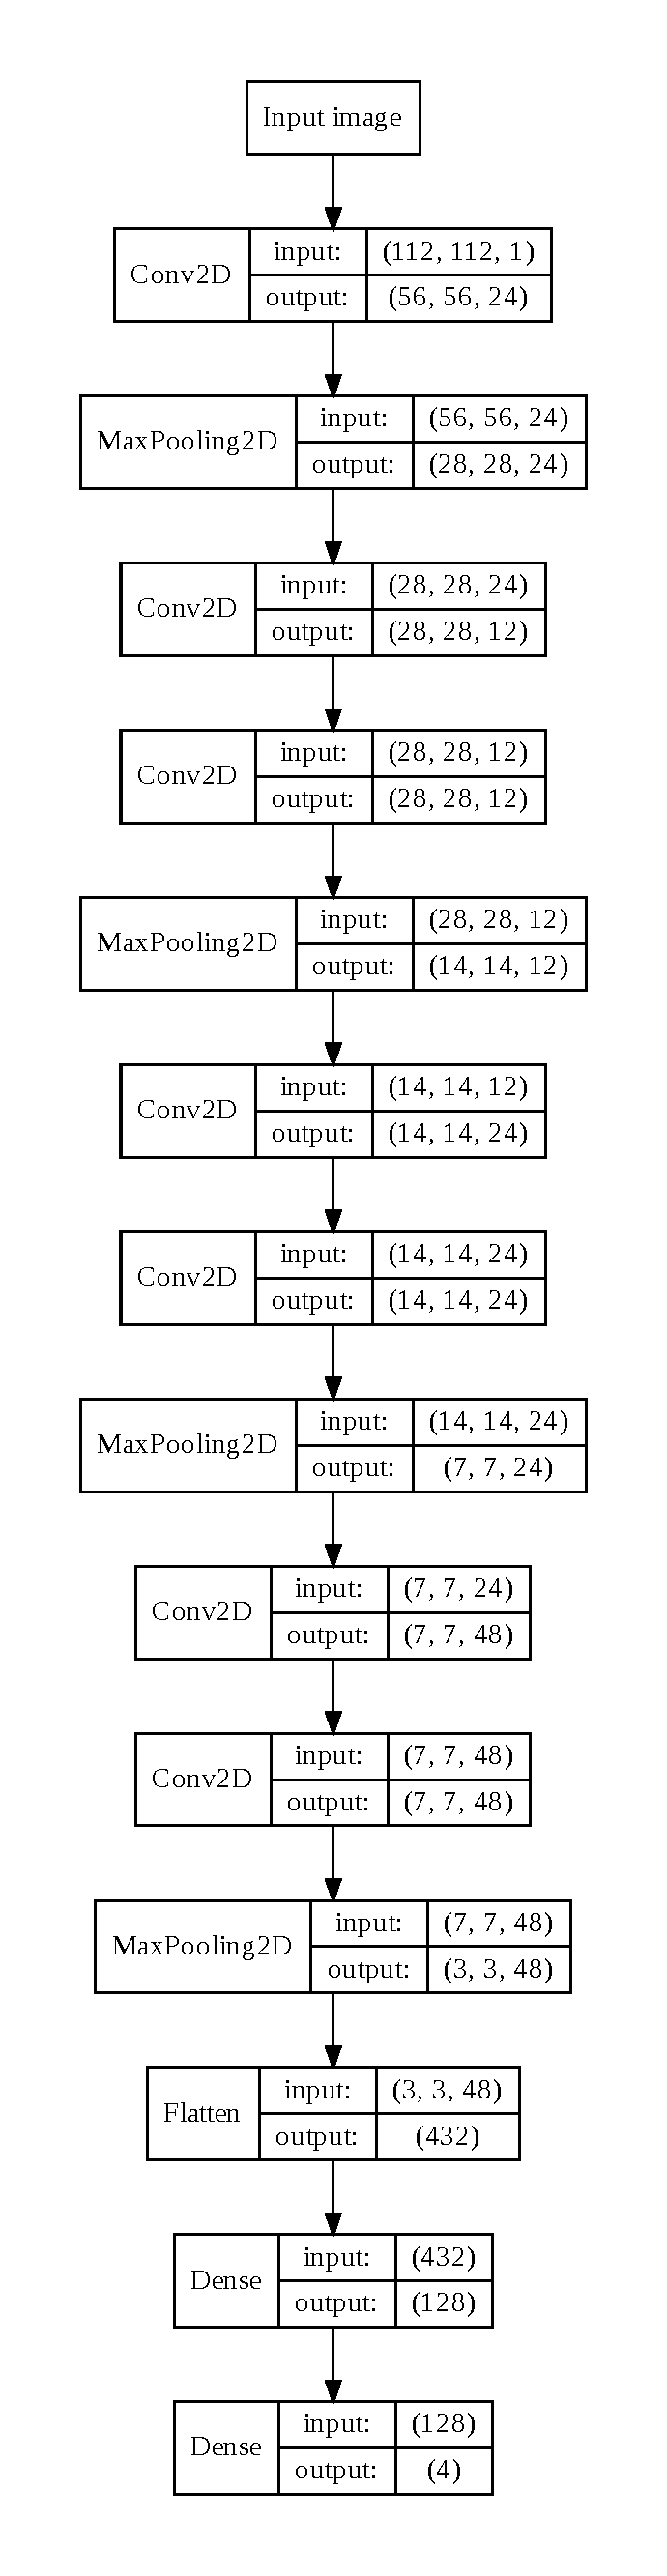
\includegraphics[width=1.7\linewidth]{img/model.pdf}
\end{wrapfigure}

We will recreate the convolutional neural network (CNN) setup used in the study by Islam and Zhang, using the machine learning framework Keras. The network will be trained and evaluated on the OASIS-3 dataset. This dataset contains data from over 2000 MRI sessions and 1000 patients, as well as medical evaluations of their disease state. OASIS-3 was a longitudinal study, which means that the imaging and evaluation of every patient was performed over a large span of time.

The dataset will be split into training, validation, and test sets, as done by Islam and Zhang. The CNN will never have seen the test set, and so it will be used for testing the accuracy. The study by Islam and Zhang resulted in a series of numerical values for accuracy, more specifically precision, recall, and f1 score. We will calculate the same values for our network trained on the larger dataset, and then compare our results with theirs. 

Studies using the smaller OASIS dataset often use cross-validation, where the training and validation is repeated multiple times so that every part of the data is used as validation at some point. This might not be possible for us depending on the computation time needed to train on the larger dataset, but would increase confidence in our results.

The CNN used by \textcite{islam2018early} uses a densely connected architecture that seems identical to DenseNet~\cite{huang2017densely}. DenseNet has implementations for both Tensorflow and PyTorch. A dense architecture means that each layer in the network is not just connected to the previous layer, but also to every other layer that came before it. This can speed up training and reduce overfitting by shrinking the parameter space and providing more direct connections between different parts of the network.

\textcite{islam2018early} do not use the entire 3D images obtained from the MRI scans. Instead, they take three slices of the image along different planes and patch them together into an image, which is then used as input to the model. It would be interesting to see if 3D convolutions could be useful for this problem, this is something we will look into if we have time.

\endgroup

\chapter{Results}
\begin{figure}
  \begin{center}
    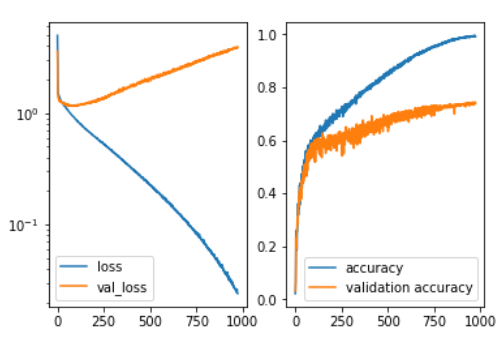
\includegraphics[width=100mm]{img/overfitted.png}
    \label{fig:overfitted}
    \caption{The result when training the network for 1000 epochs without data augmentation. (Note log scale on left diagram.)}
  \end{center}
\end{figure}
\begin{figure}
  \begin{center}
    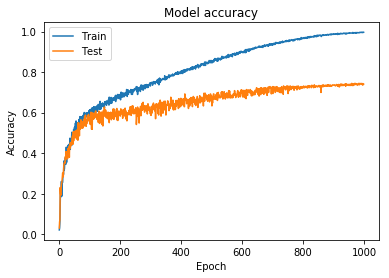
\includegraphics[width=100mm]{img/overfitted_acc.png}
    \label{fig:overfitted_acc}
    \caption{The result when training the network for 1000 epochs without data augmentation. (Note log scale on left diagram.)}
  \end{center}
\end{figure}

\begin{figure}
  \begin{subfigure}{.5\textwidth}
    \centering
    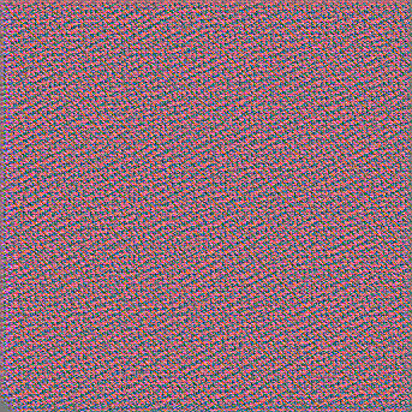
\includegraphics[width=0.9\linewidth]{img/layer0.png}
    \label{fig:layer0}
    \caption{Initial convolution}
  \end{subfigure}%
  \begin{subfigure}{.5\textwidth}
    \centering
    
\includegraphics[width=0.9\linewidth]{img/layer1.png}
    \label{fig:layer1}
    \caption{Second convolution}
  \end{subfigure}
  \\[10pt]
  \begin{subfigure}{1\textwidth}
    \centering
    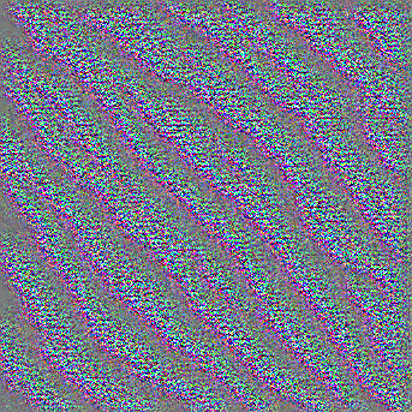
\includegraphics[width=0.45\linewidth]{img/layer2.png}
    \label{fig:layer2}
    \caption{Third convolution}
  \end{subfigure}
  \label{fig:filtervis}
  \caption{Selected filter visualizations from the first three convolution layers.}
\end{figure}

The learning rate of the Adam optimizer was found to be very important for good results. The default learning rate of $0.001$ appears to be to large, and the result was the network not improving. A lower rate of $10^{-5}$ resulted in more and faster improvement during training.

\section{Initial training}
At first, the network reached an accuracy of around 78~\% in a single epoch. Further training did not let the network progress.
Training the data with all classes equally, results in the op

Validating on 555 images...
              precision    recall  f1-score   support

           0       0.85      0.88      0.86       422
           1       0.39      0.32      0.35        96
           2       0.30      0.29      0.29        35
           3       0.00      0.00      0.00         2

   micro avg       0.74      0.74      0.74       555
   macro avg       0.38      0.37      0.38       555
weighted avg       0.73      0.74      0.74       555

\chapter{Discussion}
Just as in the study by \textcite{islam2018early}, the low frequency of samples in the dataset showing progressed dementia is an issue. Thanks to OASIS-3 containing many times the number of MRI images as the original OASIS does, this is not too large of a problem during training, The low frequency is however very noticible during validation, when it results in single-digit counts of the rarest class (\textit{moderate dementia}). This gives very rough knowledge of how accurate the model actually is on this type of data. It might be useful to increase the ratio of validation to training data, and in the long term create new and larger datasets that enables researchers to evaluate their models' performance with more confidence. On the other hand, detecting these progressed cases of dementia might no be very useful in practice, since by then the symptoms will be so pronounced that the diagnosis can not be missed.

\section{Method}
\section{Results}

\chapter{Conclusions}

% Print the bibliography (and make it appear in the table of contents)
\printbibliography[heading=bibintoc]

\appendix


% Tailmatter inserts the back cover page (if enabled)
\tailmatter

\end{document}
